\documentclass{article}
\usepackage{authblk}
\usepackage{graphicx}
\usepackage{subcaption}
\usepackage{float}
\usepackage{multicol}

\title{\textbf{Examen Práctico}}
\author[1]{Manuel Olmos Antillón --- A01750748}
\affil[1]{Ingeniería en Sistemas Computacionales 5° semestre, Escuela de Ingeniería y Ciencias, Tecnológico de Monterrey}
\date{\today}

\begin{document}

\maketitle
\tableofcontents

\section{ITC}
\indent \indent Para contarles acerca de cómo llegué hasta aquí, debo retroceder un poco en el tiempo y hablarles de cómo mis sueños y esperanzas se vieron afectadas por mis decisiónes.
Con el paso de los años, mi interés por ayudar a las personas fue creciendo, y con ello, mi deseo de estudiar medicina, por lo que consulté mi primer libro\cite{alvarez2020}. Sin embargo, al llegar a la preparatoria, me di cuenta de que el esfuerzo que hacía no era el suficiente.
Siempre fui muy conformista en cuanto a mis calificaciones, y eso me llevó a no esforzarme lo suficiente para lograr el promedio que necesitaba para estudiar medicina. 
Pocos meses antes de salir de preparatoria, probé hacer el examen de medicina para el Campus Ciudad de México del Tecnológico de Monterrey; mis esperanzas se desvanecieron en cuanto un coordinador me marcó para decirme que no daba la talla para estudiar medicina.
Después de eso, me sentí muy desanimado y sin rumbo. No sabía qué hacer con mi vida, y me sentía muy perdido.

\indent Fue entonces cuando me incliné por la Tecnología y empecé a estudiar estructuras de datos\cite{stephens2013essential}, mi deseo de ayudar a las personas estaba más fuerte que nunca y sabía que aunque no estudiaría medicina, podría hacer grandes cambios en la sociedad, estuviera donde fuera.
Posteriormente llegaron materias extraordinarias que me ayudaron en la toma de decisiones para mi desarrollo como programador (ver Tabla \ref{tab:tabla1}). % chktex 2
Sin embargo, no todo es color de rosa, ya que llegaron las ecuaciones diferenciales y las matemáticas avanzadas, materias que me hicieron dudar de mi capacidad para seguir adelante. Las ecuaciones que me hicieron llorar son de la materia de física las cuales explican el comportamiento de los fluidos (ver Ecuación \ref{eq:continuidad1} \ref{eq:continuidad2} y Ecuación \ref{eq:bernoulli}). % chktex 2

\indent Ecuación de continuidad:
\begin{equation}
    V_{1a} \cdot S_{1b} = V_{2a} \cdot S_{2b}
    \label{eq:continuidad1}
\end{equation}
\begin{equation}
    \sum_{i=1}^n {(V_{i1} \cdot S_{i2})}_{\mathrm{entrantes}} = \sum_{j=1}^m {(V_{j1} \cdot S_{j2})}_{\mathrm{salientes}}
    \label{eq:continuidad2}
\end{equation}

\indent Ecuación de Bernoulli:
\begin{equation}
    P_1 + \frac{1}{2} \rho v_1^2 + \rho g h_1 = P_2 + \frac{1}{2} \rho v_2^2 + \rho g h_2
    \label{eq:bernoulli}
\end{equation}

\begin{figure}[H]
    \centering
    \begin{subfigure}[b]{0.45\textwidth}
        \centering
        
\includegraphics[scale=0.25,angle=0]{doctor.png}
        \caption{Portada del libro: Pero querías ser doctor}\label{fig:doctor}
    \end{subfigure}
    \hfill
    \begin{subfigure}[b]{0.45\textwidth}
        \centering
        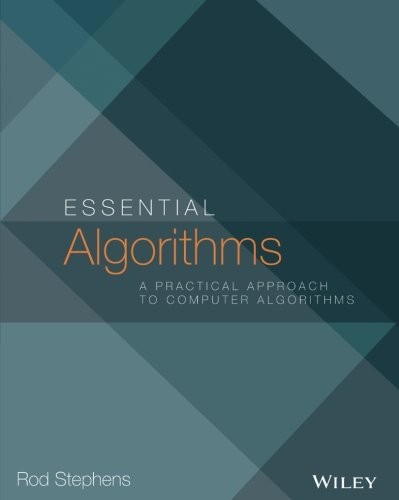
\includegraphics[scale=0.385, angle=0]{stephens.jpg}
        \caption{Portada del libro de Stephens (2013)}\label{fig:stephens2013}
    \end{subfigure}
\end{figure}

\begin{table}[H]
    \centering
    \begin{tabular}{|c|c|} % chktex 44
        \hline % chktex 44
        \textbf{Materia} & \textbf{Semestre} \\
        \hline % chktex 44
        Analysis and Design of Advanced Algorithms & 5°  \\
        \hline % chktex 44
        TC2007B.401: Aplicación Móvil para Socio Formador & 5° \\
        \hline % chktex 44
        Data structures with C++ & 3° \\
        \hline % chktex 44
    \end{tabular}
    \caption{Tabla que describe las materias más importantes de mi carrera}\label{tab:tabla1}
\end{table}

\section{Conclusión}
En esta sección voy a redactar mis conclusiones y comentarios finales.

\subsection{Planes Futuros}
\begin{multicols}{2}
    Al finalizar mi carrera, tengo varios objetivos tanto en el ámbito laboral como académico. En el ámbito laboral, me gustaría trabajar en una empresa de tecnología donde pueda aplicar mis conocimientos en desarrollo de software y algoritmos avanzados. Estoy particularmente interesado en trabajar en proyectos que involucren inteligencia artificial y aprendizaje automático, ya que considero que estas áreas tienen un gran potencial para transformar diversas industrias.

    En el ámbito académico, planeo continuar mis estudios y obtener una maestría en ciencias de la computación tanto como el doctorado posteriormente. Me gustaría especializarme en áreas como la ciberseguridad o la ciencia de datos, ya que creo que estas disciplinas serán cruciales en el futuro. Además, me gustaría participar en proyectos de investigación y contribuir al avance del conocimiento en estas áreas.
\end{multicols}

\bibliographystyle{plain}
\bibliography{ExamenRefs}


\end{document}